\documentclass[10pt]{article}

\usepackage{graphicx}
\usepackage{times}
\usepackage[T1]{fontenc}
\usepackage{amsmath}
\usepackage[ngerman]{babel}
\usepackage[ansinew]{inputenc}
\usepackage{fixltx2e}
\usepackage{setspace}
\usepackage{geometry}
\usepackage{amsthm}
\usepackage{cite}
\usepackage{url}
%\usepackage{multirow}
\geometry{a4paper,left=30mm,right=30mm, top=3cm, bottom=3cm}
\newcommand{\result}[1]{\underline{\underline{#1}}}
%\usepackage{mathtools}
%\usepackage{dingbat}
%\usepackage{bbding}
\usepackage{amssymb}
\usepackage{amsfonts}
\newcommand{\ol}[1]{\overline{#1}}
\newcommand{\varrule}[2]{#1& $\longrightarrow$ & #2\\}
\newcommand{\predic}[2]{\mbox{\textit{#1}}(\mbox{\textit{#2}})}

\title{How-To GIT for \textbf{\texttt{s0pra}} \texttt{v1.1}}
\author{Sascha Rechenberger\\sascha.rechenberger@uni-ulm.de}

\begin{document}
\maketitle

\section{Einf�hrung}
	Hier f�r alle, kompakt und �bersichtlich zusammengefasst, alle wichtigen Befehlsfolgen zum arbeiten mit GIT.
	
	Grunds�tzlich gilt es, folgende Reihenfolgen einzuhalten:
	\paragraph{Vorbereitung}
		\begin{verbatim}
			clone;
		\end{verbatim}
		
	\paragraph{Arbeitsbeginn}
		\begin{verbatim}
			pull;
		\end{verbatim}
		
		Falls beim \texttt{pull} ein Mergekonflikt auftritt, ist folgendes zu tun.		
		\begin{verbatim}
			commmit; /* Als Nachricht bitte etwas wie "Conflict fixed" */
			pull;
		\end{verbatim}			
	
	\paragraph{Arbeitsende}
		\begin{verbatim}
			gegebenenfalls: add;			
			commit;
			pull;
			push;
		\end{verbatim}
		
	Welche Aktionen die K�rzel diktieren wird im Folgenden beschrieben.
	
	Eine Nichteinhaltung f�hrt oft zu \emph{Mergekonflikten}, welche zu \emph{Fehlern in den Textdatein} f�hren k�nnen, welche \emph{\textbf{unn�tige Arbeit}} erzeugen.
	Daher bekommt der \emph{Projektverwalter} bei jedem derartigen Fehler eine Tasse Kaffee oder eine Dose Monster vom Verursacher spendiert, um genug Energie zu haben diese Fehler zu beseitigen.
		
\section{GIT-Hub f�r Windows}

	Hier folgen relativ genaue Instruktionen zum Arbeiten mit der \emph{GIT-Hub for Windows} GUI, welche hier\footnote{\url{http://windows.github.com/}} zum Herunterladen zur verf�gung steht.

	\subsection{clone}
		Um unser Repositorium zu klonen, einfach auf den eigenen Nutzernamen klicken---hier \emph{SRechenberger} (1)---und dann auf \emph{CLONE} beim entsprechenden Repositorium (2).
		\begin{center}
			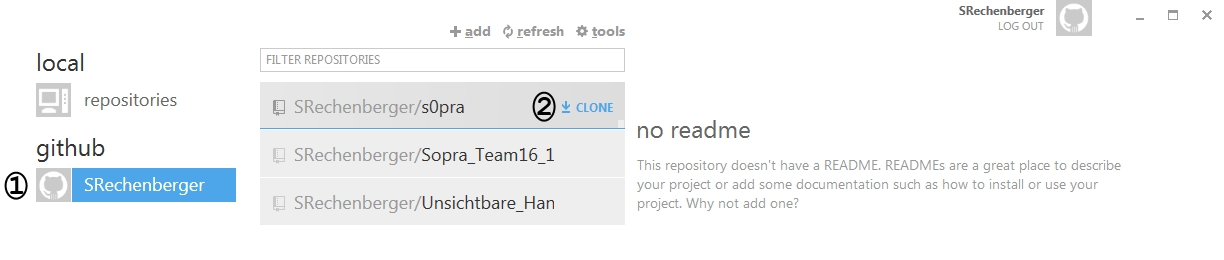
\includegraphics[width=1\textwidth]{ressources/clone.jpg}
		\end{center}
		
		Um das Repositorium dann zu �ffnen klicke man auf den kleinen Pfeil in der entsprechenden Kachel (1).
		\begin{center}
			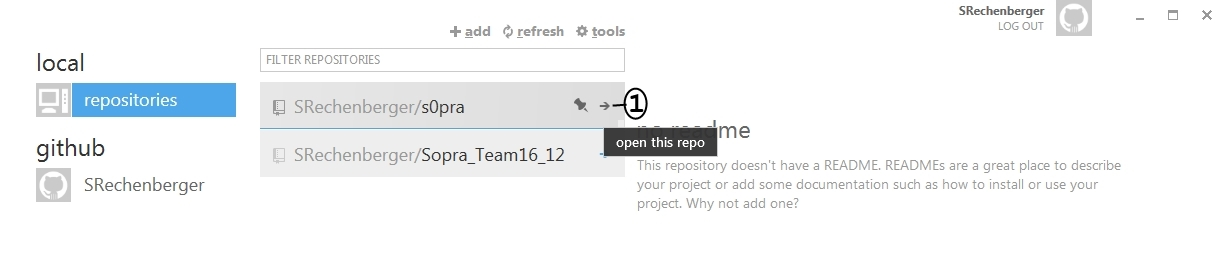
\includegraphics[width=1\textwidth]{ressources/open.jpg}
		\end{center}	
	
	\subsection{add}
		Von GIT zu verfolgende Datein kann man via An- oder Abw�hlen der entsprechenden H�ckchen hinzuf�gen oder entfernen.
		\begin{center}
			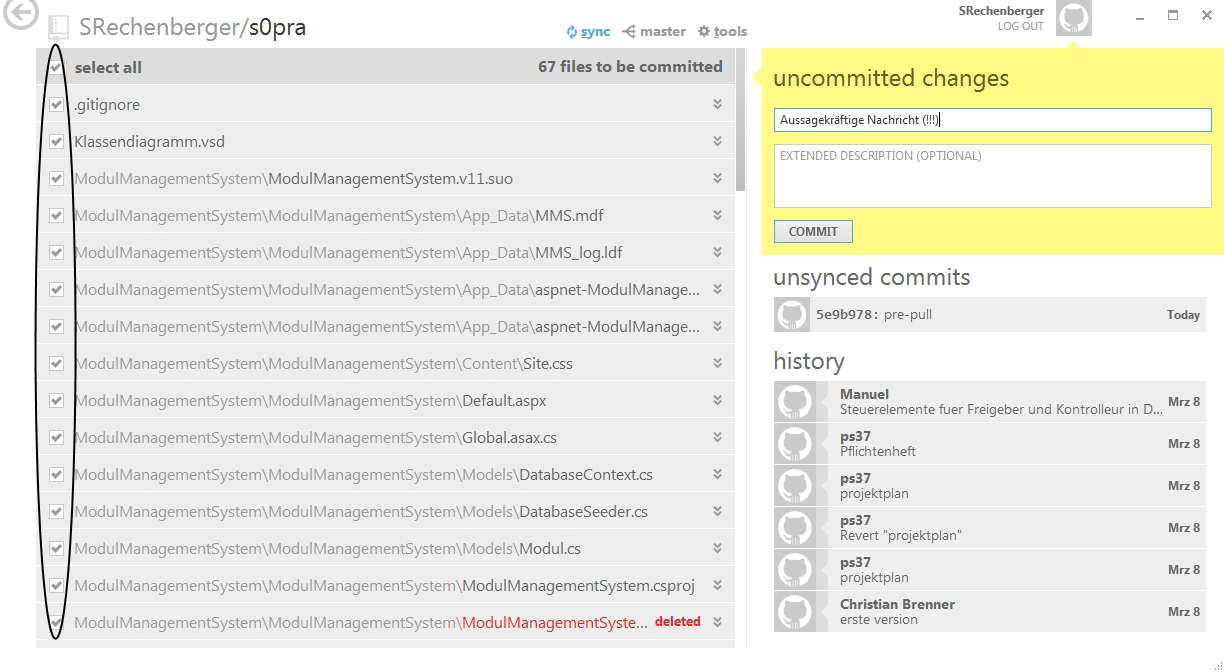
\includegraphics[width=1\textwidth]{ressources/add.jpg}
		\end{center}	
		
	\subsection{commit}			
		Um dann zu committen, gebt eine \emph{aussagekr�ftige Nachricht} bei (1) ein, klickt auf \emph{commit} (2).
		\begin{center}
			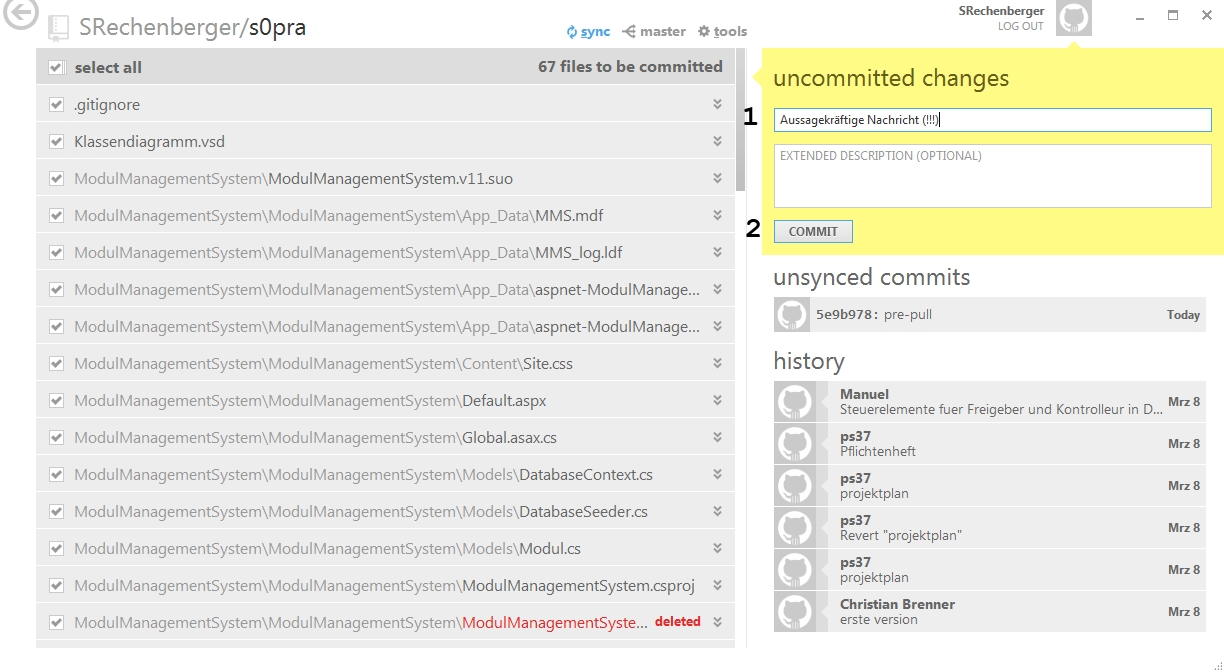
\includegraphics[width=1\textwidth]{ressources/commit.jpg}
		\end{center}
		
	\subsection{pull $\vee$ push $=$ sync}
		Um das lokale Repositorium mit dem fernen abzugleichen klicke man auf \emph{sync} (1).
		\begin{center}
			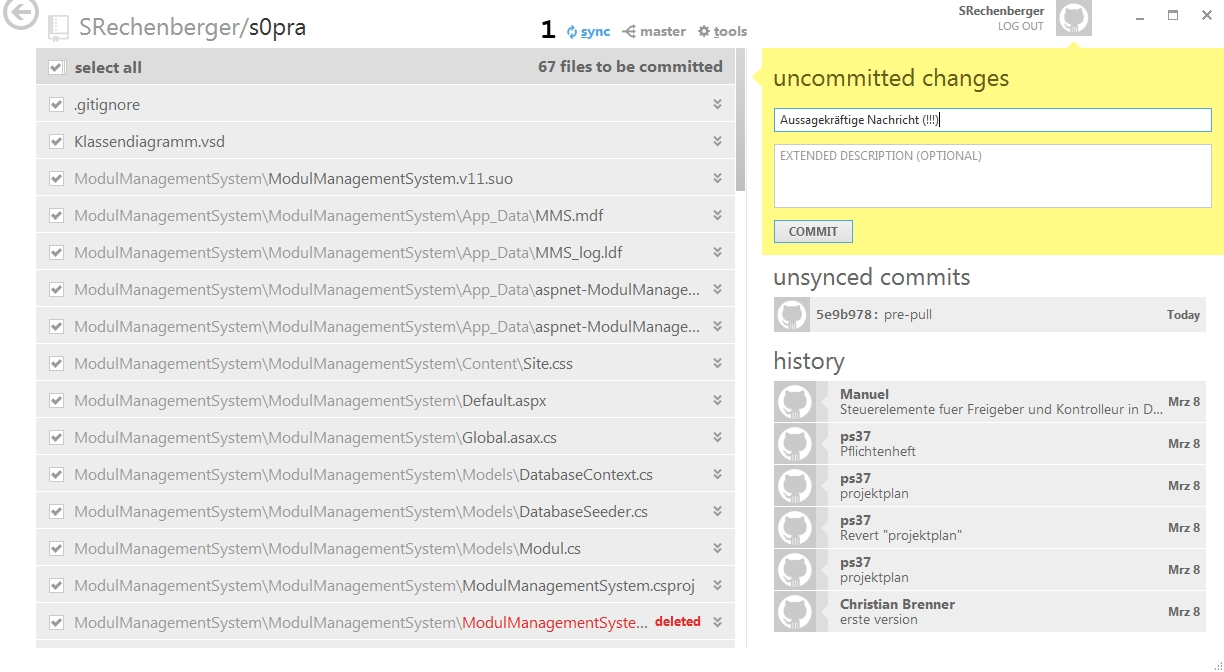
\includegraphics[width=1\textwidth]{ressources/sync.jpg}
		\end{center}	
		
	
	
\section{(GIT-)Bash}
	
	Hier folgen genaue Instruktionen zum arbeiten mit der GIT-Bash.
	Um dies zu k�nnen muss man jedoch erst die hier\footnote{\url{https://help.github.com/articles/generating-ssh-keys}} beschriebenen Schritte ausf�hren.
	Grunds�tzlich ist es n�tig zuerst via \texttt{cd <PFAD>}---sowohl unter Windows wie unter Linux---in das Verzeichnis des Repositoriums zu wechseln.
	
	\subsection{clone}	
		Zum klonen des Repositoriums in das Verzeichnis wechseln, in dem das Repositorium sich befinden soll, und dann 
		\begin{verbatim}
			git clone git@github.com:SRechenberger/s0pra
		\end{verbatim}
		eingeben.
		
	\subsection{add}	
		Um neue Dateien oder ganze Verzeichnisse von GIT verfolgen zu lassen gebe man
		\begin{verbatim}
			git add <DATEI_ODER_VERZEICHNIS>
		\end{verbatim}
		ein.
		
		Wendet man \texttt{git add} auf ein Verzeichnis an, so verfolgt GIT \emph{alle} Dateien im Verzeichnis und dessen Unterverzeichnissen.
		
	\subsection{commit}
		Um �nderungen zu committen gebe man
		\begin{verbatim}
			git commit -am "aussagekr�ftige Nachricht (!!!)"
		\end{verbatim}
		ein. Hier gilt es wieder in der Nachricht m�glichst aussagekr�ftig zu beschreiben, welche �nderungen dieser Commit mit sich bringt.
	\subsection{pull}
		Zum pullen gebe man
		\begin{verbatim}
			git pull origin master
		\end{verbatim}
		ein.
		
	\subsection{push}
		Zum pushen gebe man
		\begin{verbatim}
			git push origin master
		\end{verbatim}
		ein.
		
\section{Allgemeine Hilfe}
	Grunds�tzlich gibt f�r jeden Befehl in der GIT-Bash eine Option \texttt{git <befehl> --help}, welche eine genaue Beschreibung des Befehls anzeigt.
	Ansonsten gibt es hier\footnote{\url{http://git-scm.com/documentation}} eine ausf�hrliche Dokumentation zu GIT.
	
	Bei Unklarheiten und noch zu kl�renden Fragen schreibe man mir eine e-Mail.
\end{document}